\section{App implementation}\label{ch:app_implementation}

The prototype suffices as proof of concept.
However, the model lacks a suitable environment to be used.
The prototype applies the model and its implementation into each instance of \name{mec-2} and patches a canvas on top of the element to be able to draw.
This is not optimal, because this approach is neither flexible nor extensible.
So instead of using just the \name{mec2} HTML-element, a web application is built around it.
This web application may be used as a progressive web app to be accessed via a browser or even embedded into other third-party apps.

\subsection{Creation of a Progressive Web App}

The goal of the application is to provide a user interface where the user can work with \name{mec2} interactively, especially using hand-drawings.
This is achieved by using \name{mec2} as the base and creating an environment around this HTML-element.

Components used to create the user interface are mostly written using \name{React}. % TODO citation needed.
React is a JavaScript framework, which allows for the usage of single components, allowing standard HTML and JavaScript besides it.
This is a requirement the original \name{mec2} HTML-Component should be used without any modifications.
By using \name{materialUI}\cite{MaterialUI2020} a consistent and modern layout is created.

\subsection{Structure of the application}

\begin{figure}
    \centering
    \fbox{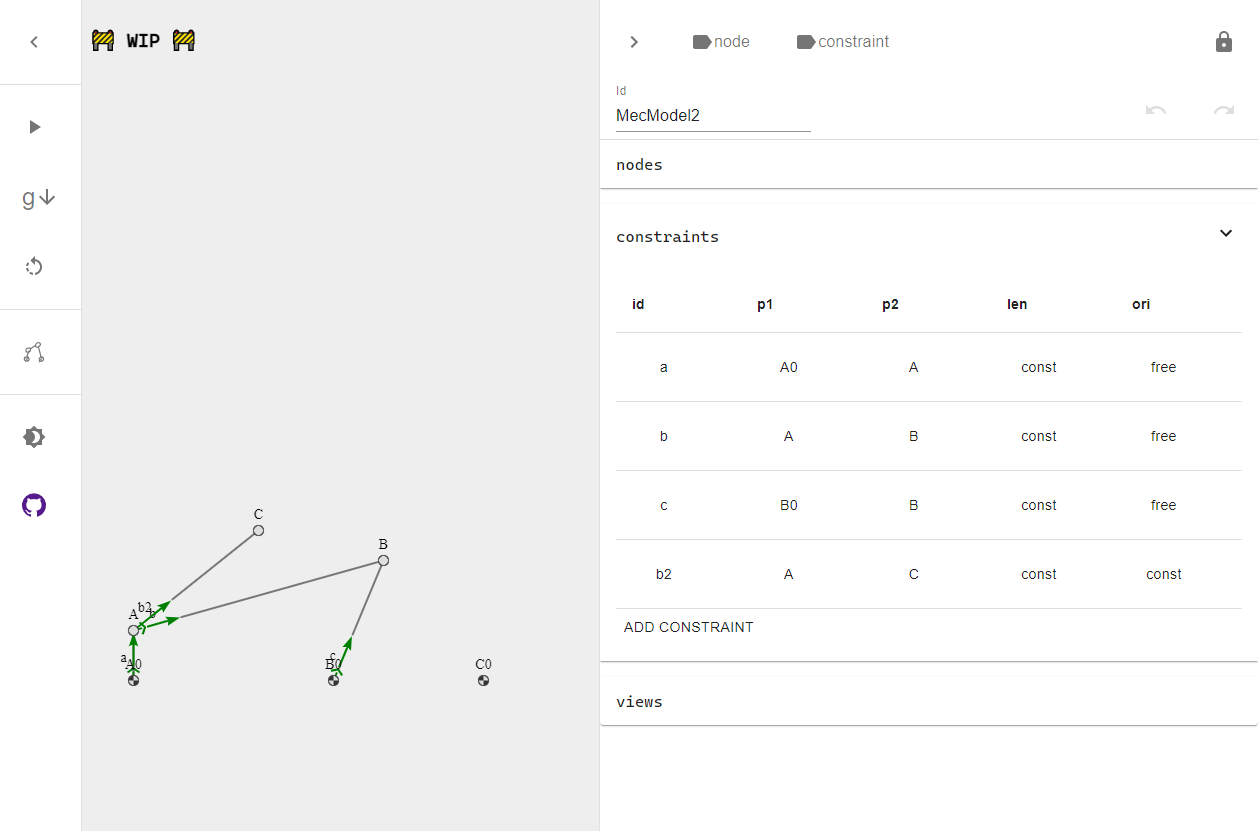
\includegraphics[width=0.8\textwidth]{images/deepmech_klawr_de.png}}
    \caption[Screenshot of the web application]{ Both drawers are expanded. On the left the \name{mec2} controls can be seen, on the right a summary of elements of the model are listed. The tab for \name{constraints} is expanded where some properties are shown }\label{fig:deepmech_klawr_de}
\end{figure}

The main part of the application is occupied by the \name{mec2} Custom HTML element.
It is stretched across the whole viewport.
On both sides are \name{Material-UI} \code{Drawer} elements, enabling the user to interact with different parts of the application.

\subsubsection{Left drawer}

The structure of the user interface aims to be simple and straight forward.
To define individual components \name{Reacts} \name{jsx} syntax is used.
\name{jsx} is a syntax very similar to \name{HTML} but with the ability to implement JavaScript into the elements\footnote{By using \name{jsx} it is now necessary to compile the project using \name{Babel.js}.}. % TODO citation neede

The left drawer contains \code{MecControl}, \code{DeepmechControl} and two other Buttons.
\code{MecControl} is a custom \name{React} component to replace the default \name{mec2} controls by using the designated API.\@

\begin{lstlisting}[label={lst:mec_control}, caption={Definition of the \name{MecControl} component.}]
export default function MecControl({ mecReset, className }) {
    const dispatch = useDispatch();
    const mec = useSelector(mecSelect);

    return <List className={className}>
        <ListButton onClick={() =>
            dispatch(mecAction.toggleRun())} tooltip="Run/Pause mechanism">
            {mec.pausing ? <PlayArrow /> : <Pause />}
        </ListButton>
        <ListButton onClick={() =>
            dispatch(mecAction.toggleGravity())} tooltip="Toggle gravity">
            g {mec.gravity ? <Clear /> : <ArrowDownward />}
        </ListButton>
        <ListButton onClick={mecReset} tooltip="Reset">
            <RotateLeft />
        </ListButton>
    </List>
}
\end{lstlisting}

Listing~\ref{lst:mec_control} shows the function which returns the component replacing the default \name{mec2} controls.
It contains the definition of the variables \code{dispatch} and \code{mec}.
\code{Selector} and \code{useDispatch} are used for state management of the user interface and are examined in Chapter~\ref{ch:state_manipulation}.
The return value of a component is the contonent defined in \name{jsx} syntax.
\code{List} is a \name{Material-UI} component.
The list items inside the list are are implemented using \code{ListItems} containing a \code{Tooltip} and an \code{IconButton}.
To reuse \name{Material-UI} components multiple times without having to call them every time a custom \code{ListButton} component is used.
The code for \code{ListButton} can be reviewed at \aka{} % TODO include link here.

The left drawer also contains the \code{DeepmechControl}\footnote{\name{deepmech} is the current project name.}.
It is responsible for handling the draw mode.
It shows the activation button if the draw mode is disabled.
If the drawing mode is enabled the left drawer does not show the \code{MecControl} anymore.
Furthermore, the \code{DeepmechControl} shows four different modes interacting with the drawing canvas.
Drawing, dragging strokes, deleting strokes, and a camera mode.
Details to the different modes and how they are implemented is explained in Chapter~\ref{ch:state_manipulation}.

The two bottom-most buttons are responsible for toggling the dark mode\footnote{The app starts in dark mode if the browser is, and vice versa.} and to navigate to the project page: \url{https://github.com/klawr/deepmech}.

\subsubsection{Right drawer}

The right drawer is intended to show all relevant information contained by the \name{mec2} model.
On the top, there are two buttons labeled \code{nodes} and \code{constraints} each with a \code{Label} icon.
Those are used to toggle the labels of \code{nodes} and \code{constraints} respectively.
The \code{Lock} Button is used to keep the drawer open when interacting with the model.
This is enabled by default if the side is wide enough; i.e.\ wider than 1200 pixels.

The last component in the \code{RightDrawer} is the \code{MecProperties} component.
The \code{MecProperties} component contains a collection of other custom components, individually created for the different properties of a \name{mec2} model.
The  first component is the \code{Id} component.
It is showing the \code{id} property of the \name{mec2} model and updates it respectively on changes.

Currently, three of the modules provided by \name{mec2} are implemented into the app:
\code{Nodes}, \code{Constraints} and \code{Views}.
They are all structured in a very similar fashion to be able to have a somewhat unified interface for the user.
To achieve that the return value of these components is very similar and can be seen in Listing~\ref{lst:mec_component_return}.

\begin{lstlisting}[label={lst:mec_component_return}, caption={Return value of a custom \name{mec2} component.}]
return <Accordion>
    <AccordionSummary> {name} </AccordionSummary>
    <AccordionDetails>
        <Grid container direction="row">
            <MultiSelect options={head} updateOptions={updateHead} />
            <MecTable
                SanitizedCell={SanitizedCell}
                head={Object.entries(head).filter(h => h[1]).map(h => h[0])}
                list={mecElement._model[name]} />
        </Grid>
    </AccordionDetails>
</Accordion>
\end{lstlisting}

The \code{Accordion} in this listing is a \name{Material-UI} component\footnote{\aka{https://material-ui.com/components/accordion/}}.
This component accepts the \code{AccordionSummary} and \code{AccordionDetails}, which are defined inside the \code{Accordion}.
In Listing~\ref{lst:mec_component_return} the \code{AccordionSummary} encapsulates the \code{name} property of the respective component, which is the name of the component in lower case; e.g. \code{const name = 'nodes'} for the \code{Nodes} component.
\code{AccordionDetails} contains elements that are shown when the \code{Accordion} is expanded.

The \code{AccordionDetails} component shows details of the respective property of the \name{mec2} model.
The \code{Grid} in the \code{AccordionDetails} in~\ref{lst:mec_component_return} contains two custom components.
\code{MultiSelect} is a dropdown menu which shows a list of the available properties of the module; e.g.\ for nodes these properties are \code{id}, \code{x}, \code{y}, \code{base}.
These properties are provided by the variable \code{head}, which is given inside the definition of the component.
This enables the possibility to show and modify other properties later on, without the necessity to show them from the start\footnote{To show all possible properties directly would also result in a very unclear user interface.}.
The \code{head} variable is a list of properties which is further discussed in Chapter~\ref{ch:state_mec2_model}.

The \code{MecTable} component is responsible for rendering the table where the properties are shown.
\code{MecTable} returns a predefined layout of a regular \code{Table} element of \name{Material-UI}, which can be reviewed at \aka{https://material-ui.com/components/tables/}.
The \code{TableHead} in \code{MecTable} contains a mapping of the different properties which are provided by \code{head} to show the properties which are shown by each column.
The rows of the table are filled using yet another custom component which is injected into the \code{MecTable}, called \code{SanitizedCell}.
\code{SanitizedCell} itself is provided by the encompassing component.
It provides information on how the individual properties are to be rendered.
The respective return value of the \code{SanitizedCell} function can be seen in Listing~\ref{lst:sanitized_cell}.

\begin{lstlisting}[label={lst:sanitized_cell}, caption={Return value of the \code{Node} components \code{SanitizedCell} function.}]
return <ContextMenu key={idx}>
    {select()}
    <MenuItem onClick={removeNode}>
        {`Remove node ${elm['id']}`}
    </MenuItem>
\end{lstlisting}

\code{select} returns the respective function based on a switch statement, which can be seen in~\ref{lst:sanitized_cell_select}.

\begin{lstlisting}[label={lst:sanitized_cell_select}, caption={Shortened version of \code{select} function inside of the \code{SanitizedCell} function of the \code{Node} component.}]
function select() {
    switch (property) {
        case 'base':
            const [checked, changeChecked] = React.useState(!!elm[property]);
            return <Checkbox checked={checked} onChange={(e) => {
                    changeChecked(e.target.checked);
                    update(e.target.checked);}} />
        case 'x':
        case 'y':
            return <UpdateText
                title={property}
                value={Math.round(elm[property])}
                onSubmit={v => update(+v)} />
        case 'id': /*...*/
        default: return <div>{elm[property]}</div>
}
\end{lstlisting}

\code{SanitizedCell} is called with an argument object containing \code{property}, \code{idx} and \code{elm}.
The \code{property} corresponds to the current value of \code{head}, which is mapped in the \code{MecTable} to fill the \code{TableRow}\footnote{Yet another property of \code{Table} which is responsible for the design of the table-rows.}.
Based on the \code{property} value the \code{select} function returns the component designed for the specific property.
If the property is equal to \code{'base'} the return value is \name{Material-UI}s \code{Checkbox}.
For textual inputs the custom component \code{UpdateText} is created, which handles updates reliably to be translated to the \name{mec2} model and back.
It is therefore used by number value like \code{'x'} and \code{'y'} or textual value like \code{'id'}.

Another custom component, which is used inside a \code{SanitizedCell} component is \code{RadioSelect}.
This custom component is used to get a selection of items and hold one as the selected item; e.g.\ constraints inside a \name{mec2} model reference two nodes, which are selected via their respective \code{id} property.
This component allows to list all nodes by their \code{id} property and select one respectively.

\subsubsection{The canvas}

As mentioned above, the viewport is occupied by the \name{mec2} Custom HTML element.
The prototype used the canvas of this HTML element to be able to draw.
This approach is cumbersome because the corresponding event handlers had to be activated and deactivated manually, which gives a lot of room for error and is not a very flexible approach.

In unison with the rest of the application, this canvas is now remodeled into a custom component.
This \code{DeepmechCanvas} component does not return a \name{React} component, but a HTML canvas, as demonstrated in Listing~\ref{lst:deepmech_canvas}.

\begin{lstlisting}[label={lst:deepmech_canvas}, caption={Return of the \code{DeepmechCanvas} component.}]
return <canvas
    id="{id}" className={classes.drawCanvas}
    width={globalThis.innerWidth} height={globalThis.innerHeight}
    ref={canvasRef} />
\end{lstlisting}

The \code{id} property is set to be able to refer to this canvas from other components.
The \code{DeepmechControl} component uses this \code{id} to be able to get access to the HTML element and forward it to the \code{predict} function.

\code{width} and \code{height} are taken from the \code{globalThis}\footnote{\aka{https://developer.mozilla.org/en-US/docs/Web/JavaScript/Reference/Global_Objects/globalThis}} property.

The \code{DeepmechCanvas} component has a \code{canvasRef} variable which is initially set to \code{const canvasRef = React.useRef(null)}.
Every time the \code{DeepmechCanvas} component is rendered the \code{canvasRef} is updated by the \code{ref} property of the returned HTML element.
See \aka{https://reactjs.org/docs/hooks-reference.html\#useref} for more information about \code{React.useRef}.

% TODO Because the reference is created after initialization, \name{Reacts} \code{useEffect}\footnote{\aka{https://reactjs.org/docs/hooks-reference.html\#useeffect}} has to be used.
\code{DeepmechCanvas}' \code{useEffect} is shown in Listing~\ref{lst:deepmech_canvas_use_effect}.

\begin{lstlisting}[label={lst:deepmech_canvas_use_effect}, caption={The \code{useEffect} function in the \code{DeepmechCanvas} component.}]
React.useEffect(() => {
    const [nl, cl] = [mec.nodeLabels, mec.constraintLabels];
    dispatch(mecAction.toggleNodelabels(false));
    dispatch(mecAction.toggleConstraintlabels(false));
    dispatch(UiAction.right(false));
    const ctx = canvasRef.current.getContext('2d');
    return handleInteractor(ctx, deepmech.mode, placeholder, () => {
        dispatch(mecAction.toggleNodelabels(nl));
        dispatch(mecAction.toggleConstraintlabels(cl));
    });
}, [deepmech.mode]);
\end{lstlisting}

The second argument (\code{[deepmech.model]}) is an array that defines the properties on which changes are monitored.
Every time a change is registered, the function which is given as the first argument is issued.

The first argument given to this function is also called after the component is rendered the first time.
This behavior is necessary because the canvas has to be initialized for the context of the canvas element to be set via \code{canvasRef.current.getContext('2d')}.
The \code{dispatch} calls set certain values which will be further examined in Chapter~\ref{ch:state_manipulation}.
Returned is a \code{handleInteractor} function.

The \code{handleInteractor} function handles the interaction of the user with the canvas.
It creates a new instance on the \code{canvasInteractor}\footnote{The \code{canvasInteractor} is discussed in Chapter~\ref{ch:canvas_interactor}} for the given \code{ctx}.
As with \code{mec2}, the global \code{canvasInteractor} is used here.

For the selection of individual \name{g2}-elements a \code{selector} variable is set to \code{g2.selector(interactor.evt)}.
The respective event listeners are defined for five different events as described in Listing~\ref{lst:handle_interactor_event_listeners}.

\begin{lstlisting}[label={lst:handle_interactor_event_listeners}, caption={Definition of event listeners on the \code{canvasInteractor}.}]
const o = { tick, pointerdown, pointerup, drag, click: pointerup }
Object.entries(o).forEach(e => interactor.on(...e));
\end{lstlisting}

The event listeners have respective functions that handle the event based on the current \code{mode} which is inserted by the function call\footnote{Every time the mode changes the function is called again, as described in the array which is given as the second argument to the \code{React.useEffect} function.}.

For example the \code{pointerdown} function, as described in Listing~\ref{lst:handle_interactor_pointerdown} contains a switch-statement handling events when the \code{mode} is set to \code{'draw'} or \code{'delete'}.

\begin{lstlisting}[label={lst:handle_interactor_pointer_down}, caption={\code{pointerdown} function in \code{handleInteractor}.}]
function pointerdown(e) {
    switch (mode) {
        case 'draw':
            // Set ply and add to command queue
            ply = {
                pts: [{ x: e.x, y: e.y }],
                lw: '2', ls: '#fff', lc: 'round', lj: 'round',
                get sh() { return this.state & g2.OVER ? plyShadow : false; }
            };
            placeholder.ply.ply(ply);
            break;
        case 'delete':
            // Filter selected node from commands array
            placeholder.ply.commands = placeholder.ply.commands.filter(
                cmd => cmd.a !== selector.selection);
            selector.evt.hit = false; // selector gets confused
            selector.selection = false; // overwrite selection
            break;
    }
}
\end{lstlisting}

The \code{ply} variable is a placeholder which is filled by the various event handlers to represent the currently drawn \code{g2.ply} element.

The \code{handleInteractor} function returns a function shown in Listing~\ref{lst:handle_interactor_return}.

\begin{lstlisting}[label={lst:handle_interactor_return}, caption={Return value of \code{handleInteractor}.}]
return () => {
    Object.entries(o).forEach(e => interactor.remove(...e));
    canvasInteractor.remove(interactor);

    fn();
}
\end{lstlisting}

This function is called by \code{useEffect} when the respective \code{DeepmechCanvas} is deleted\footnote{Which is also done if it is rerendered.}.
It reverts the changes made to the \code{canvasInteractor} and also calls \code{fn} which is a function given as argument.
\code{fn} is injected because it needs access to the scope in which the \code{dispatch} and \code{mecAction} resides, as seen in Listing~\ref{lst:deepmech_canvas_use_effect}.

\subsection{State manipulation}\label{ch:state_manipulation}
\subsection{State of the \name{mec2} model}\label{ch:state_mec2_model}

The state of the elements of the user interface is controlled by the 
